
\documentclass[man,natbib,floatsintext]{apa7}
\usepackage[american]{babel}
\usepackage{microtype}
\usepackage{amsmath}
\usepackage{booktabs}
\usepackage{float}
\usepackage{graphicx}
\usepackage{url}
\usepackage{amsfonts}

\begin{document}

\subsection{Entropy}

The entropy has a significant increase after the manipulation. While in both cases, before and after manipulation, entropy decays with time (pearson $r=-0.292$ and $-0.0066$ respectively, $p-value<0.01$), it is significantly more stable during the manipulation phase. Also, it can be observed an abrupt increase in the entropy after the manipulation, denoting the rapid induced need for searching the position of the attributes. A sensitivity test was conducted, calculating the difference between the entropy taking a window from 1 to 50 trials before and after the manipulation. The result is shown in the following figure. It can be seen that the difference is significant considering a window of up to 50 trials before and after the manipulation. On the long run, it is likely the attention will fall to previous levels.
\begin{figure}[H]
    \centering
    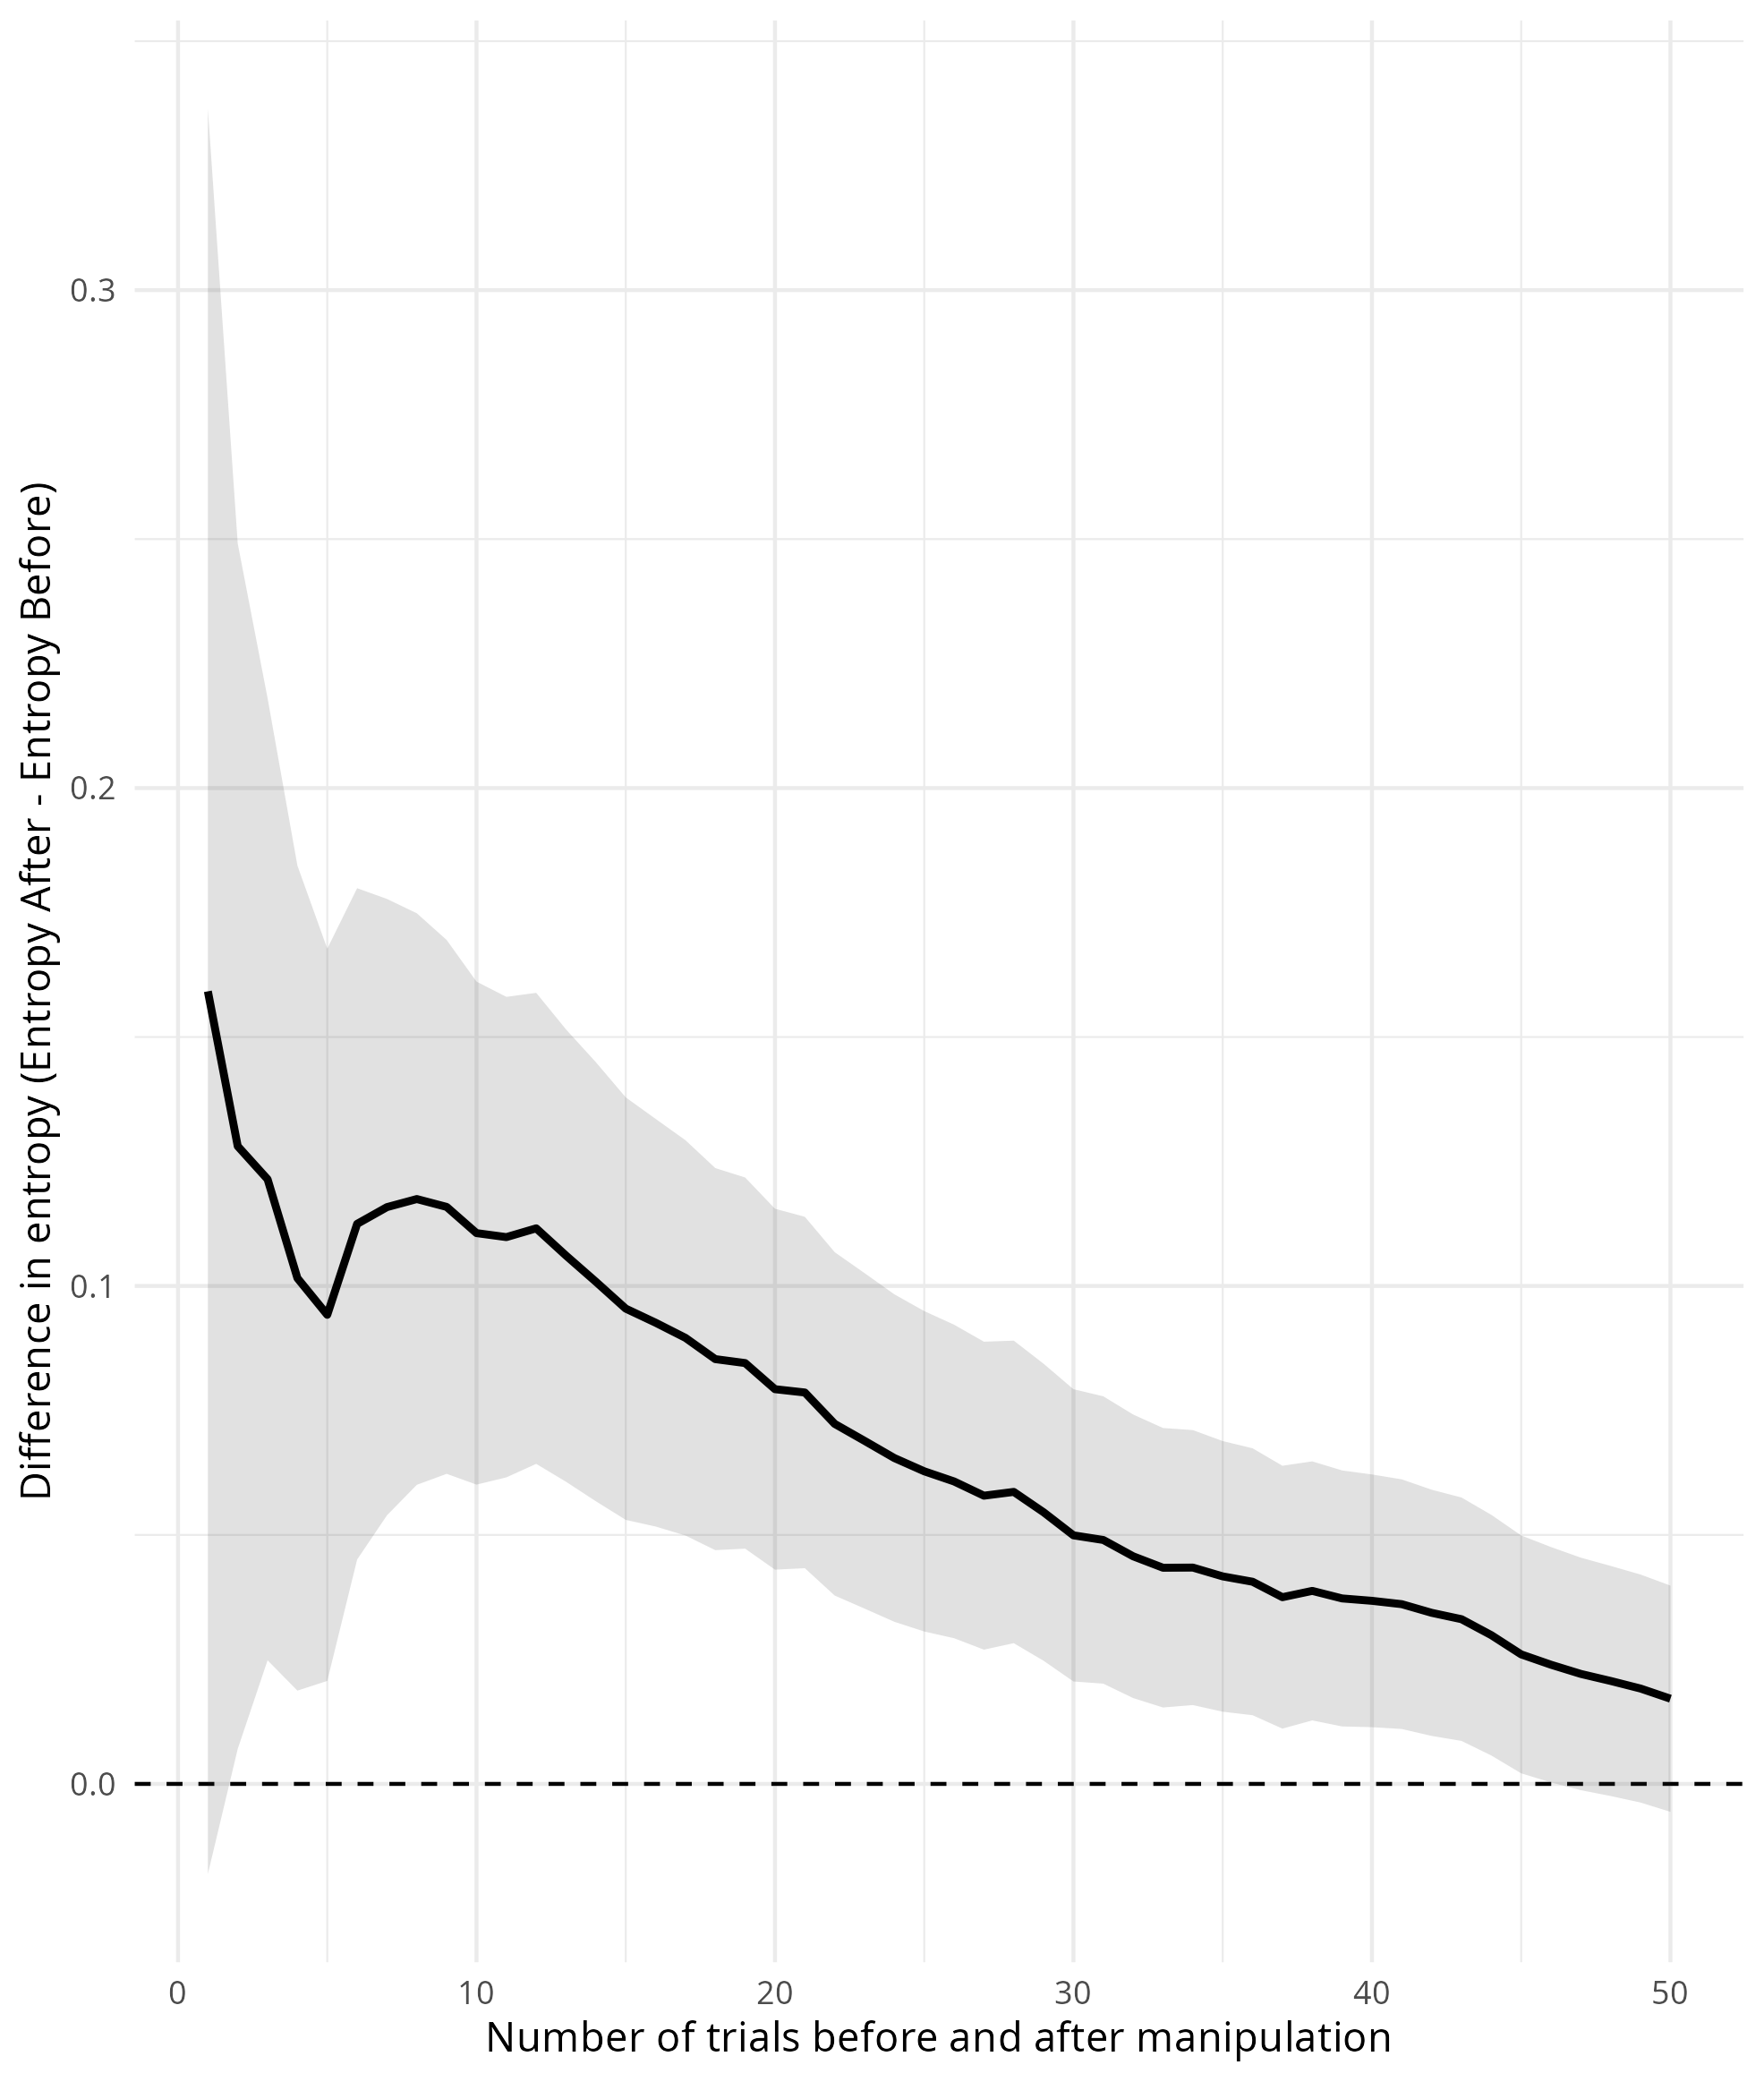
\includegraphics[width=0.75\linewidth]{Figures/sensitivity_entropy.png}
    \caption{Entropy difference sensitivity test}
    \label{fig:entropy}
\end{figure}


\subsection{Response time}
The response time immediately after the manipulation are significantly higher than before the manipulation. The first 20 trials after the manipulation have an average response time between 0.69 and 2.46 s higher than the 20 trials before the manipulation for the online sample ($p-value=0.05$), and between 1.18 and 2.89 s higher in the in-lab sample ($p-value=0.05$). A sensitivity test was conducted taking between 1 and 50 trials before and after manipulation. The following figure show the average difference and the CI 95\% for each case. The response time differences are higher in the immediate interface around the manipulation. It vanishes on the long run, meaning that after the manipulation the response time goes back to average values.
\begin{figure}[H]
    \centering
    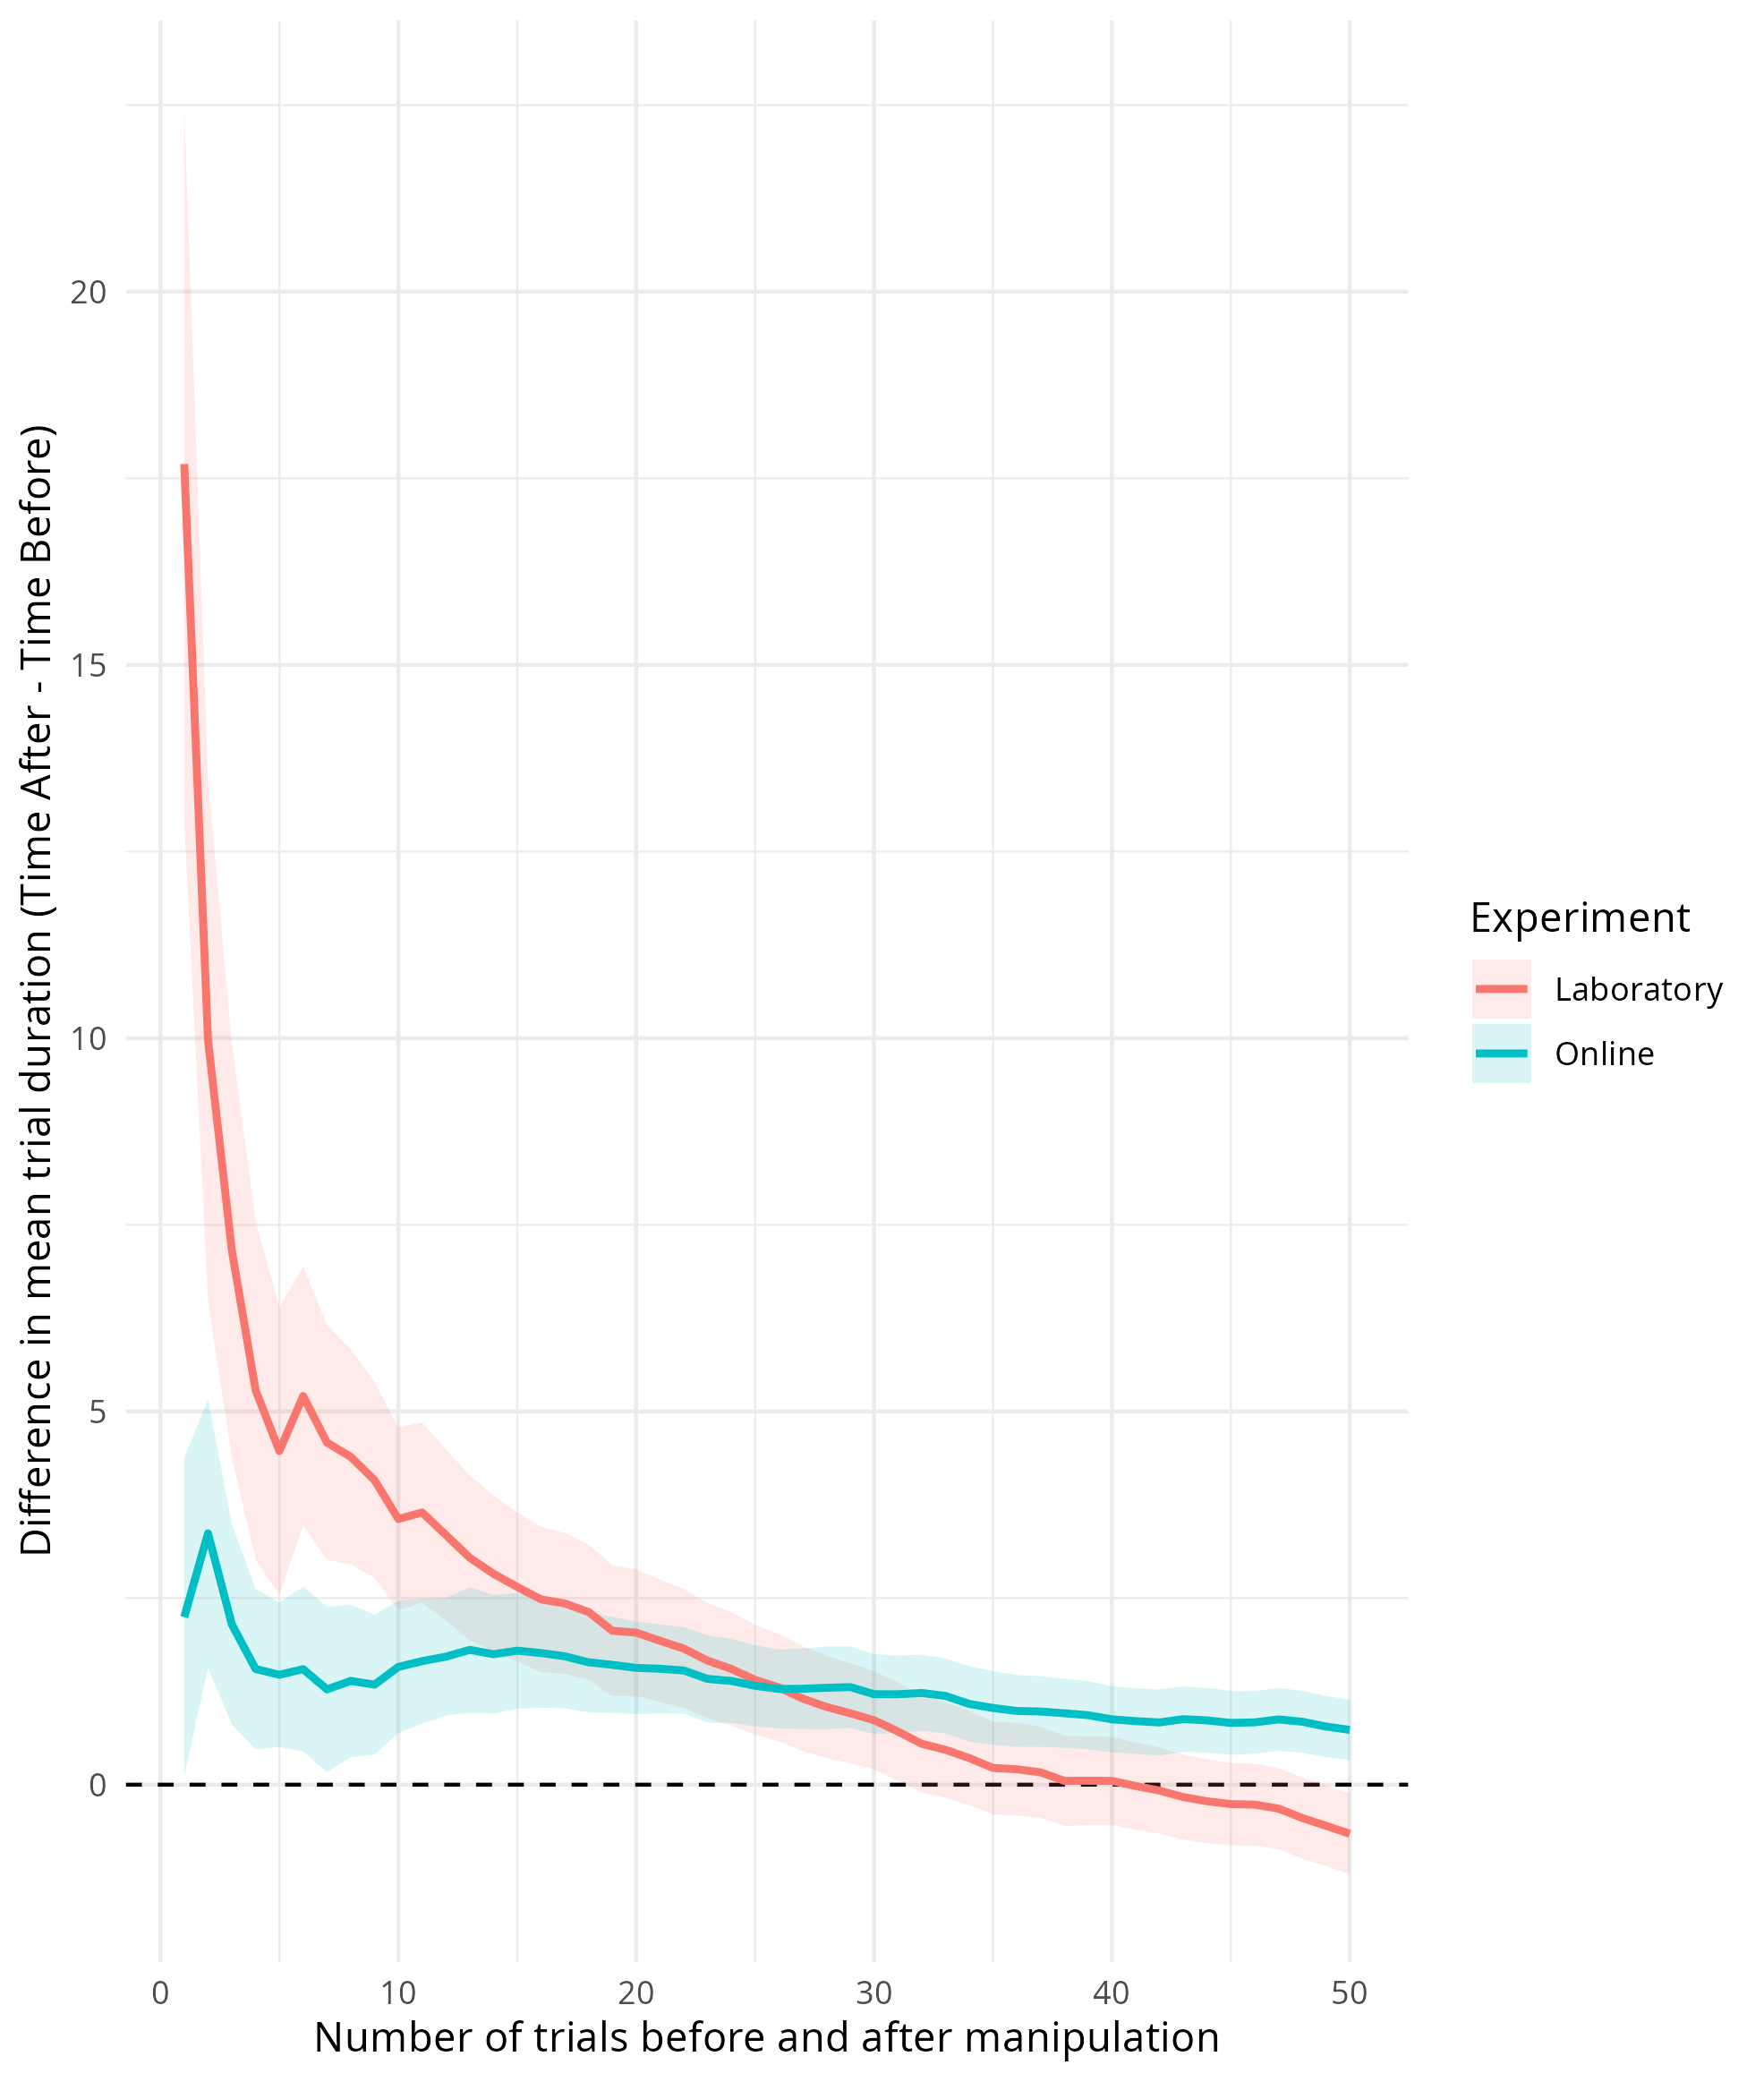
\includegraphics[width=0.8\linewidth]{Figures/sensitivity_resp_time.png}
    \caption{Sensitivity test response time differences}
    \label{fig:sensitivity}
\end{figure}

\subsection{Probability of stay}
We run a formal test to see whether individuals became habitual during the first phase and whether this is reverted with the manipulation. First, the intuition is the following. Obviously, it is expected that the choice to be repeated if the past alternative is still the best option. However, if the individual repeats the same choice when the alternative is not the best option among the set, then he/she is likely to be under habitual control. We first define the probability of staying with the same option as $P^{stay}_{nt}=\mathbf{P}(y_{n,t,i}=y_{n,t-1,i}|y_{n,t-1,i}=1)$.

Then, the formal test to see whether an individual $n$ runs under habitual control in trial $t$ is to see if the probability of staying with the same alternative given that the alternative is not the best is higher after training than before training. 

% That, is habits hold if 
% $(P^{stay}_{nt}|V_{nti}<\max{V_{ntj}}, i\neq j)>(P^{stay}_{nt'}|V_{nt'i}<\max{V_{nt'j}}, i\neq j)$, with $t>t'$ and $y_{n,t-1,i}=1$.

To do this, we run the following beta regression (beta regression is necessary since the dependent variable is bounded between 0 and 1). We test the effect of trials ($t$), manipulation ($M_{nt}$), the value of the previously chosen alternative ($\delta_{nt}=1$ if $V_{it}< \max{V_{jt}}$ and 0 in other case, with $y_{it-1}=1$)  and their interactions. Under this notation $\delta_{nt}$ indicates whether the alternative chosen in $t-1$ is now worse than the other alternatives in time $t$, under the subjective parameters of individual $n$. We allow the regression to have random inter-individual intercepts:

\begin{align}
P^{stay}_{nt} &\sim \operatorname{Beta}\!\left(\mu_{nt}\phi,\,
(1-\mu_{nt})\phi\right), \\[4pt]
\log\left(\frac{\mu_{nt}}{1-\mu_{nt}}\right)
&=
\beta_0
+ b_{nt}
+ \beta_{\delta} \delta_{nt}
+ \biggl[\beta_{t} t+\beta_M M_{nt}
+ \beta_{t \times  M} (t \times M_{nt}) \biggr]\notag\\
&\quad
+ \biggl[\beta_{t\times \delta} t+\beta_{M \times \delta } (M_{nt})
+ \beta_{t \times  M \times \delta} (t \times M_{nt}) \biggr]\times \delta_{nt}  ,
\\[4pt]
b_{nt} &\sim \mathcal{N}(0,\sigma_b^2),
\end{align}

where,

\begin{itemize}
    \item $P^{stay}_{nt}$ is the probability of staying for participant $n$ at trial $t$;
    \item $\mu_{nt} = \mathbb{E}[P^{stay}_{nt}]$;
    \item $\delta_{nt} = 1$ if the previous alternative is not the best ($V_{it}< \max{V_{jt}}, with y_{it-1}=1$), and $0$ otherwise;
    \item $M_{nt}=1$ if $t>100$ and 0 other case, indicates the post-intervention period;
    \item $b_{nt}$ is a participant-specific random intercept;
    \item $\phi$ is the beta-distribution precision parameter.
\end{itemize}

First, the $\beta_{\delta}$ should be negative since it is expected that, given that the past alternative is not the best ($\delta_{nt}=1$), the stay probability should be lower. Then, if the behavior becomes habitual during the first phase, $\beta_t$ should be negative, meaning that the probability of repeating the choice decreases even  given that the previous option is still the best. Similarly, the effect $\beta_{t\times \delta}$ should be positive if the individuals are under habitual behavior (it becomes more likely to repeat the choice when the alternative is not the best). Then, to test if habits are reverted after the manipulation, the $\beta_M$ and $\beta_{M\times \delta}$ should be analyzed. The first parameter should be positive, i.e. the likelihood of choosing the same alternative when it is the best option goes back to normal levels (expected to be high), and the second parameter should be negative, indicating that the probability of stay goes back to low levels. 

The following table shows the estimates of the regression. All the expected effects are verified. That is, individuals become more habitual with training ( $\beta_{t}=-0.004, \beta_{t\times \delta}=0.0067,\,p-value<0.001$), and the habitual behavior is reverted with the manipulation ($\beta_{M}=0.299,\,p-value=0.0546,\text{ and } \beta_{M\times \delta}=-0.4543,\, p-value<0.05$).

\begin{table}[htbp]
\centering
\caption{Regression estimates and model fit statistics}
\label{tab:regression_results}
\begin{tabular}{lrrrr}
\hline
\textbf{Variable} &
\textbf{Estimate} &
\textbf{Std. Error} &
\textbf{$z$ value} &
\textbf{$p$-value} &
\hline
Intercept
    & $1.1270$
    & $0.0267$
    & $42.14$
    & $<0.001$\\
$(\delta_{nt}=1)$ 
    & $-2.8130$
    & $0.0357$
    & $-78.87$
    & $<0.001$\\
Trial 
    & $-0.0040$
    & $0.0004$
    & $-9.16$
    & $<0.001$\\
Manipulation 
    & $0.2998$
    & $0.1559$
    & $1.92$
    & $0.0546$\\

Trial $\times$ Manipulation
    & $0.0001$
    & $0.0013$
    & $0.07$
    & $0.9413$\\

Trial $\times$ $(\delta_{nt}=1)$
    & $0.0067$
    & $0.0006$
    & $11.39$
    & $<0.001$\\

Manipulation $\times$  $(\delta_{nt}=1)$ 
    & $-0.4543$
    & $0.2116$
    & $-2.15$
    & $0.0318$\\
Trial $\times$ Manipulation $\times$ $(\delta_{nt}=1)$
    & $-0.0006$
    & $0.0018$
    & $-0.33$
    & $0.7396$\\
\hline
\multicolumn{5}{l}{\textit{Model fit statistics}} \\
\hline
\multicolumn{2}{l}{AIC}
    & \multicolumn{3}{r}{$-20{,}428.5$} \\

\multicolumn{2}{l}{BIC}
    & \multicolumn{3}{r}{$-20{,}351.1$} \\

\multicolumn{2}{l}{Log-likelihood}
    & \multicolumn{3}{r}{$-10{,}224.2$} \\

\multicolumn{2}{l}{$R^2$}
    & \multicolumn{3}{r}{$0.868$} \\

\hline
\multicolumn{5}{l}{
\footnotesize
\textit{Notes:} 
*** $p<0.001$;
** $p<0.01$;
* $p<0.05$;
$\cdot$ $p<0.10$.
} \\
\end{tabular}
\end{table}

\subsection{Attention on dominant AOI}

The share of attention received by the dominant AOI drops after the manipulation. That is, the relative attention received by the AOI with the highest fixation time—defined as the ratio between fixation time and trial duration—decreases when the choice context becomes unstable. Considering only the 20 trials before and after the manipulation, we estimate that, on average, the dominant AOI receives between 1.73\% and 3.36\% less visual attention ($p\text{-value}=0.05$). This indicates that attention becomes more evenly distributed. However, when considering only the trial immediately before and the first trial after the manipulation, the difference reaches up to 6\% of trial duration. It should be noted that the experiment includes 19 AOIs: 4 attribute labels, 3 alternative labels, and 12 attribute values. Therefore, a completely even distribution of visual attention would correspond to 5.26\% of attention per AOI. Thus, changes on the order of 3-6\% are therefore considerable in magnitude.

As in the previous analyses, we conduct a sensitivity analysis by varying the estimation window from 1 to 50 trials before and after the manipulation (\autoref{fig}). Even when considering a window of 50 trials, the estimated difference remains negative and statistically significant.

\begin{figure}
    \centering
    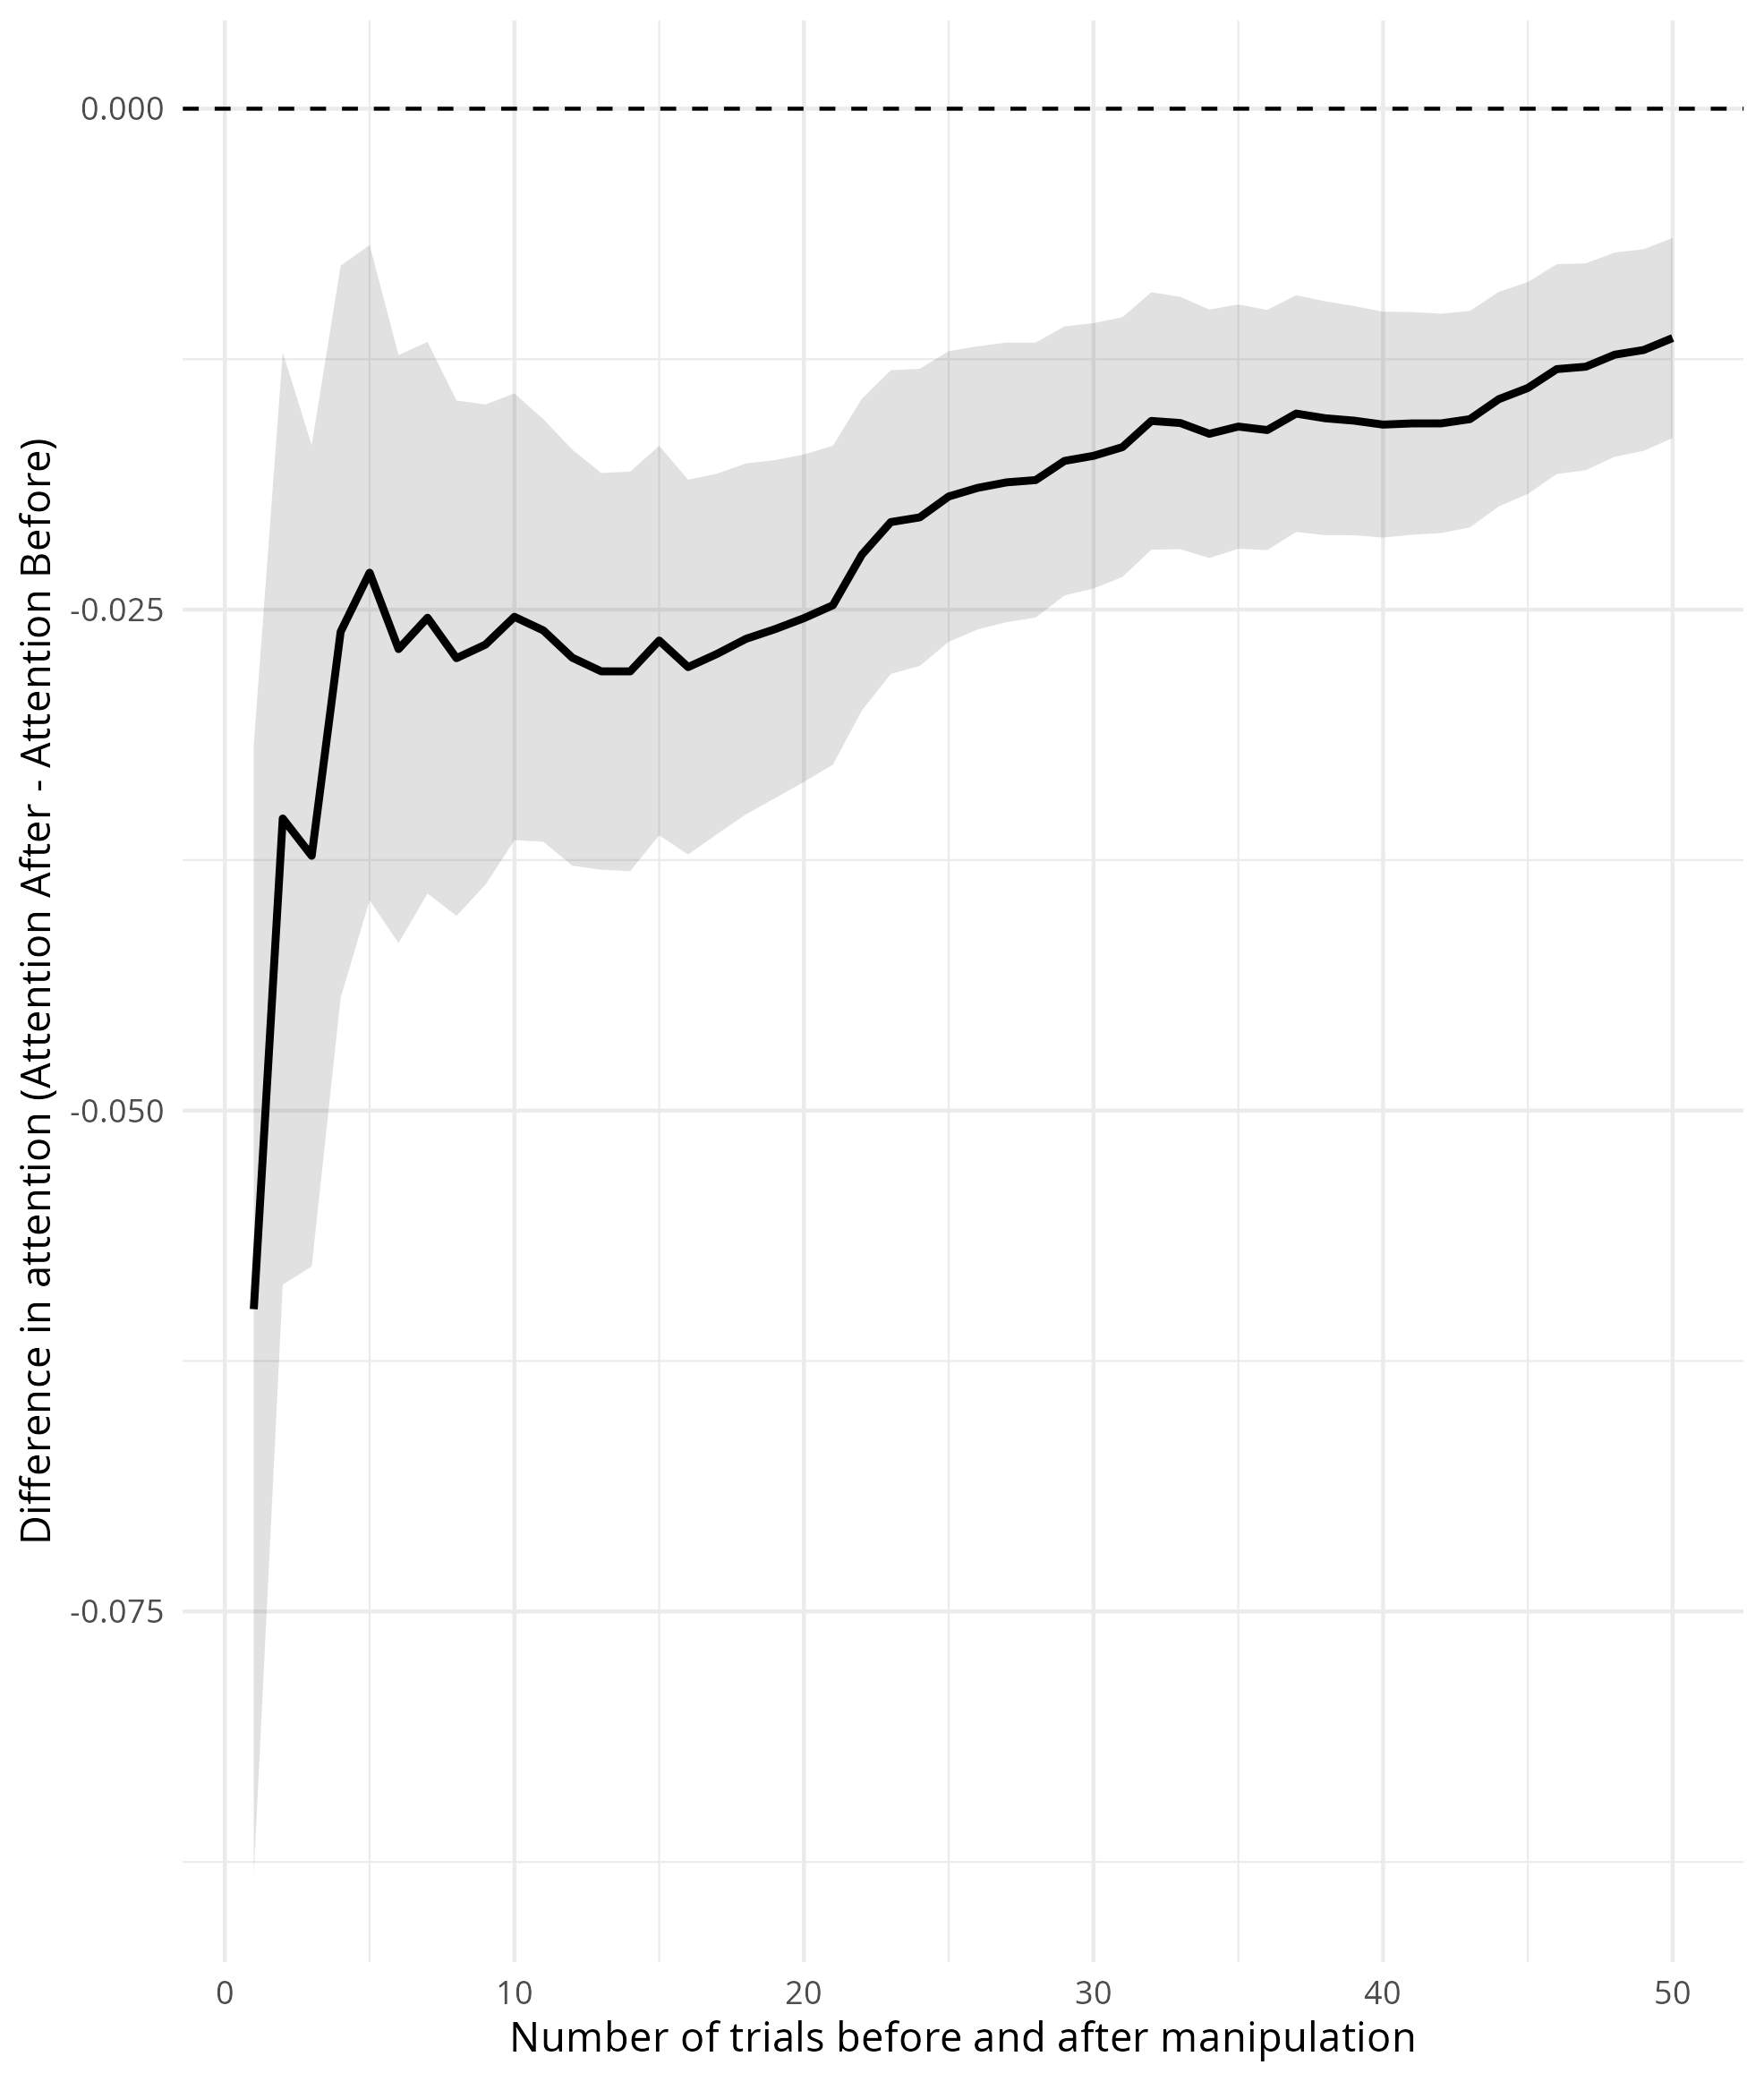
\includegraphics[width=0.75\linewidth]{Figures/sensitivity_dominant_AOI.png}
    \caption{Sensitivity test share dominant attention}
    \label{fig:dominant_AOI}
\end{figure}

\subsection{Parameters and inertia change}

 We calculated the relative change in each parameter by dividing its estimate at each trial $t$ by its estimate in the first trial. This measure indicates how much each parameter increases or decreases over time. Interestingly, during the training phase all attribute parameters decreased over time at the same rate, whereas the inertia parameter increased. For all attribute parameters, the correlation between the relative scale and trial number was $r=-0.5689,,p<0.001$. The inertia parameter increased at a similar rate, showing a positive correlation with trial number of $r=0.542,,p<0.001$. This suggests that, as inertia gains importance in the decision process, the weight of all attributes decreases, which may be interpreted as a signal that the habitual system is gaining behavioral control. However, after the manipulation the parameters are much less dependent on time, which is evidence of higher behavioral stability caused by the manipulation.


\begin{table}[htbp]
\centering
\caption{Correlation between parameter scales and trial number before and after the manipulation}
\label{tab:beta_trial_correlations_period}
\begin{tabular}{llcc}
\toprule
Manipulation & Parameter & Correlation & $p$-value \\
\midrule
After  & CO$_2$ scale  & $-0.0864$ & $<0.001$ \\
Before & CO$_2$ scale  & $-0.5680$ & $<0.001$ \\
After  & Comfort scale & $-0.0868$ & $<0.001$ \\
Before & Comfort scale & $-0.5680$ & $<0.001$ \\
After  & Cost scale    & $-0.0866$ & $<0.001$ \\
Before & Cost scale    & $-0.5670$ & $<0.001$ \\
After  & Inertia scale & $\phantom{-}0.0822$ & $<0.001$ \\
Before & Inertia scale & $\phantom{-}0.5420$ & $<0.001$ \\
After  & Time scale    & $-0.0866$ & $<0.001$ \\
Before & Time scale    & $-0.5670$ & $<0.001$ \\
\bottomrule
\end{tabular}
\end{table}


\end{document}
